\Cref{fig:app_CO2_REF_lin} shows the yearly emissions attributed for each sector in the REF case (\ie imposed \ce{CO2}-budget) and a case where the \ce{CO2}-trajectory is constrained instead. Interestingly, these two transition pathways end up in a similar carbon-neutral whole-energy system in 2050. The two main sectors that significantly reduce their emissions in the REF case are the production of \gls{HVC} and the high-temperature heat. In the former, this is linked to the extended use of oil products through naphtha-cracking. The latter is produced by industrial coal boilers for longer, until 2040. Overall, ending up to the same level of emissions in 2050, the REF case represents a 60\% reduction of the cumulative emissions compared to the linear decrease, for a 7.5\% more expensive transition.

\begin{figure}[htbp!]
\centering
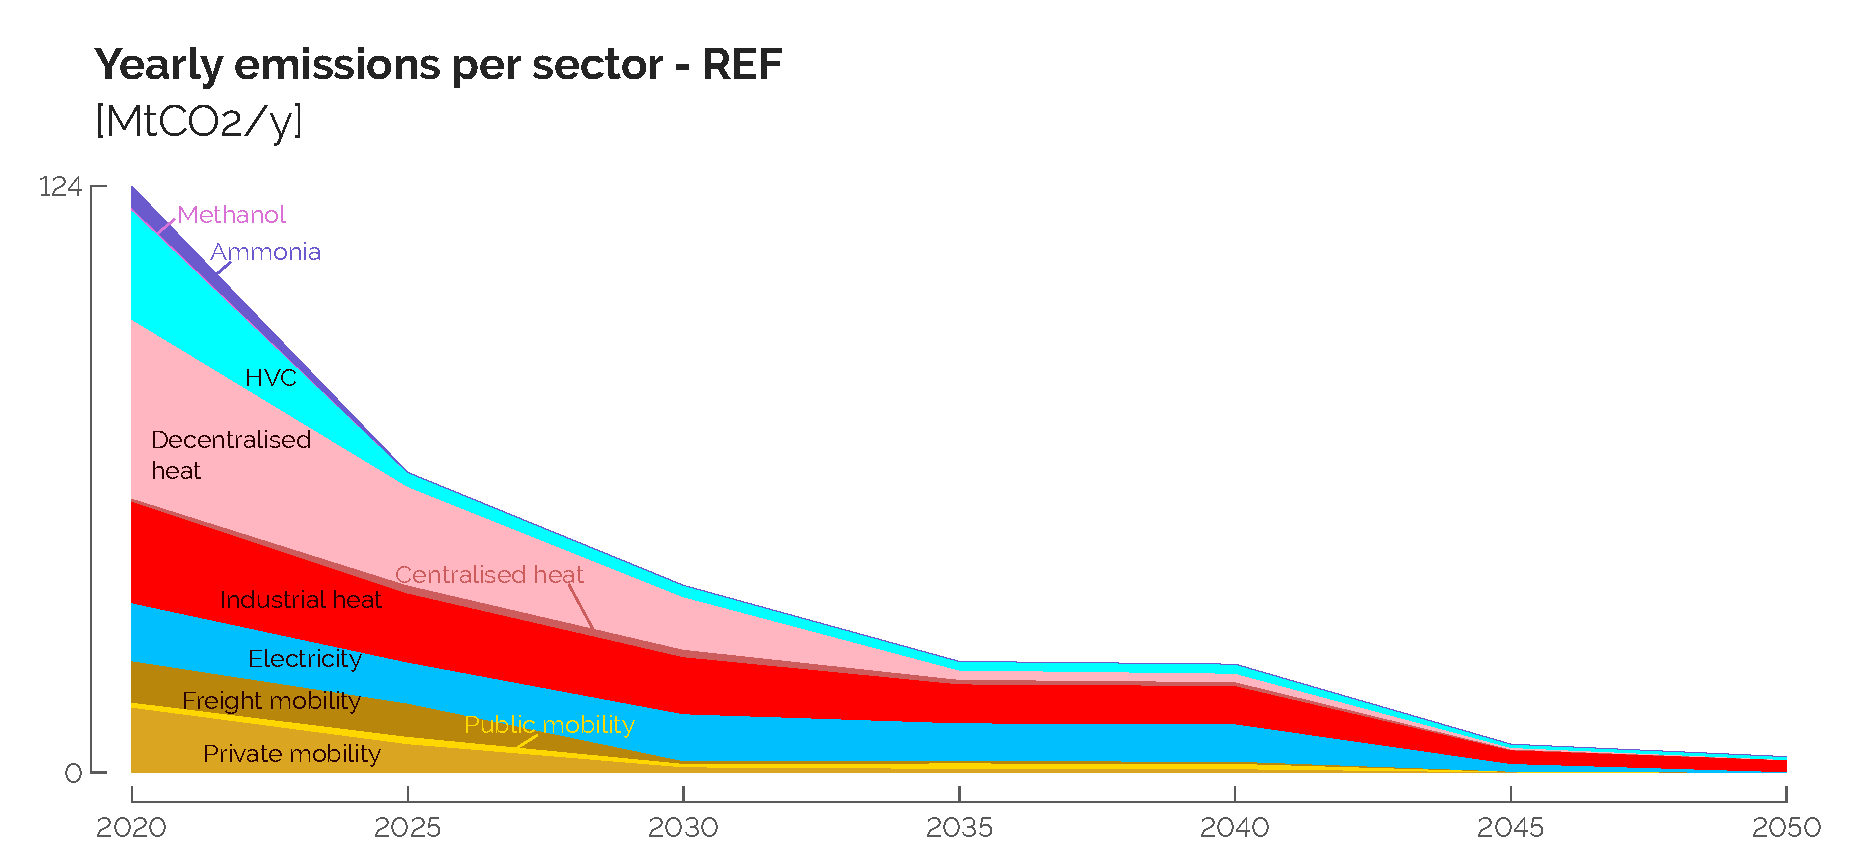
\includegraphics[width=0.49\textwidth]{GWP_per_sector_REF.pdf}
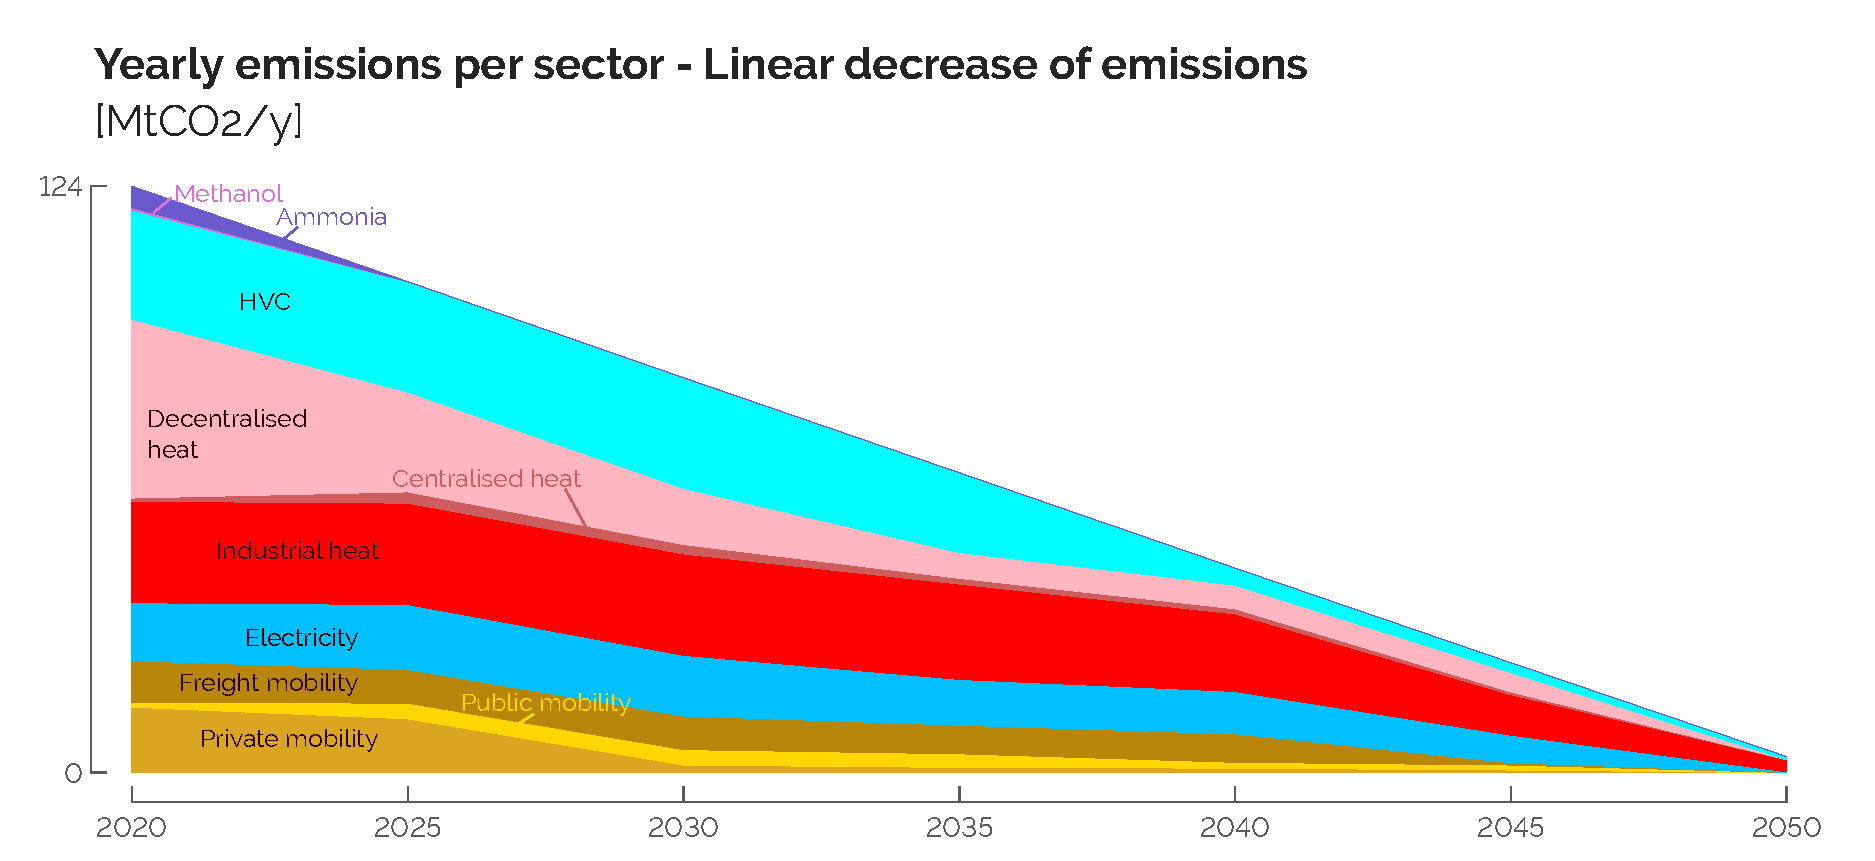
\includegraphics[width=0.49\textwidth]{GWP_per_sector_lin.pdf}
\caption{Respecting the \ce{CO2}-budget imposed in the REF case drastically cuts the emissions of the system, especially in the production of \glsxtrfull{HVC} and the high-temperature heating sector.}
\label{fig:app_CO2_REF_lin}
\end{figure}